\section{Model and Framework}
\label{sec:model_and_framework}

The first attempt is continuing using the model used by LightRel, the logistic regression model offered by LibLinear. But to form the required format that fit LibLinear is quite handy because it needs to be file format with a kind of sparse matrix representation. That become complicated when we need to do k-fold cross-validation on the training set.

Then we tried to use Scikit Learn library. Because the API of Scikit Learn are similar so we can switch from multiple models and test the performance easily. We have tried LinearSVC, LogisticRegression and Decision TreeClassifier. And we found the LogisticRegression has still had the best performance.

In the test of LightGBM, the performance is not quite ideal. In the first case, we think that because the dimension of features is too large, using a tree-based algorithm may not be a good idea.

Finally, we have tried the simple version TextCNN model, the performance is not too bad but still lower than the statistics machine learning model. So we have deprecated it later on.

\begin{figure*}[ht]
    \begin{center}
    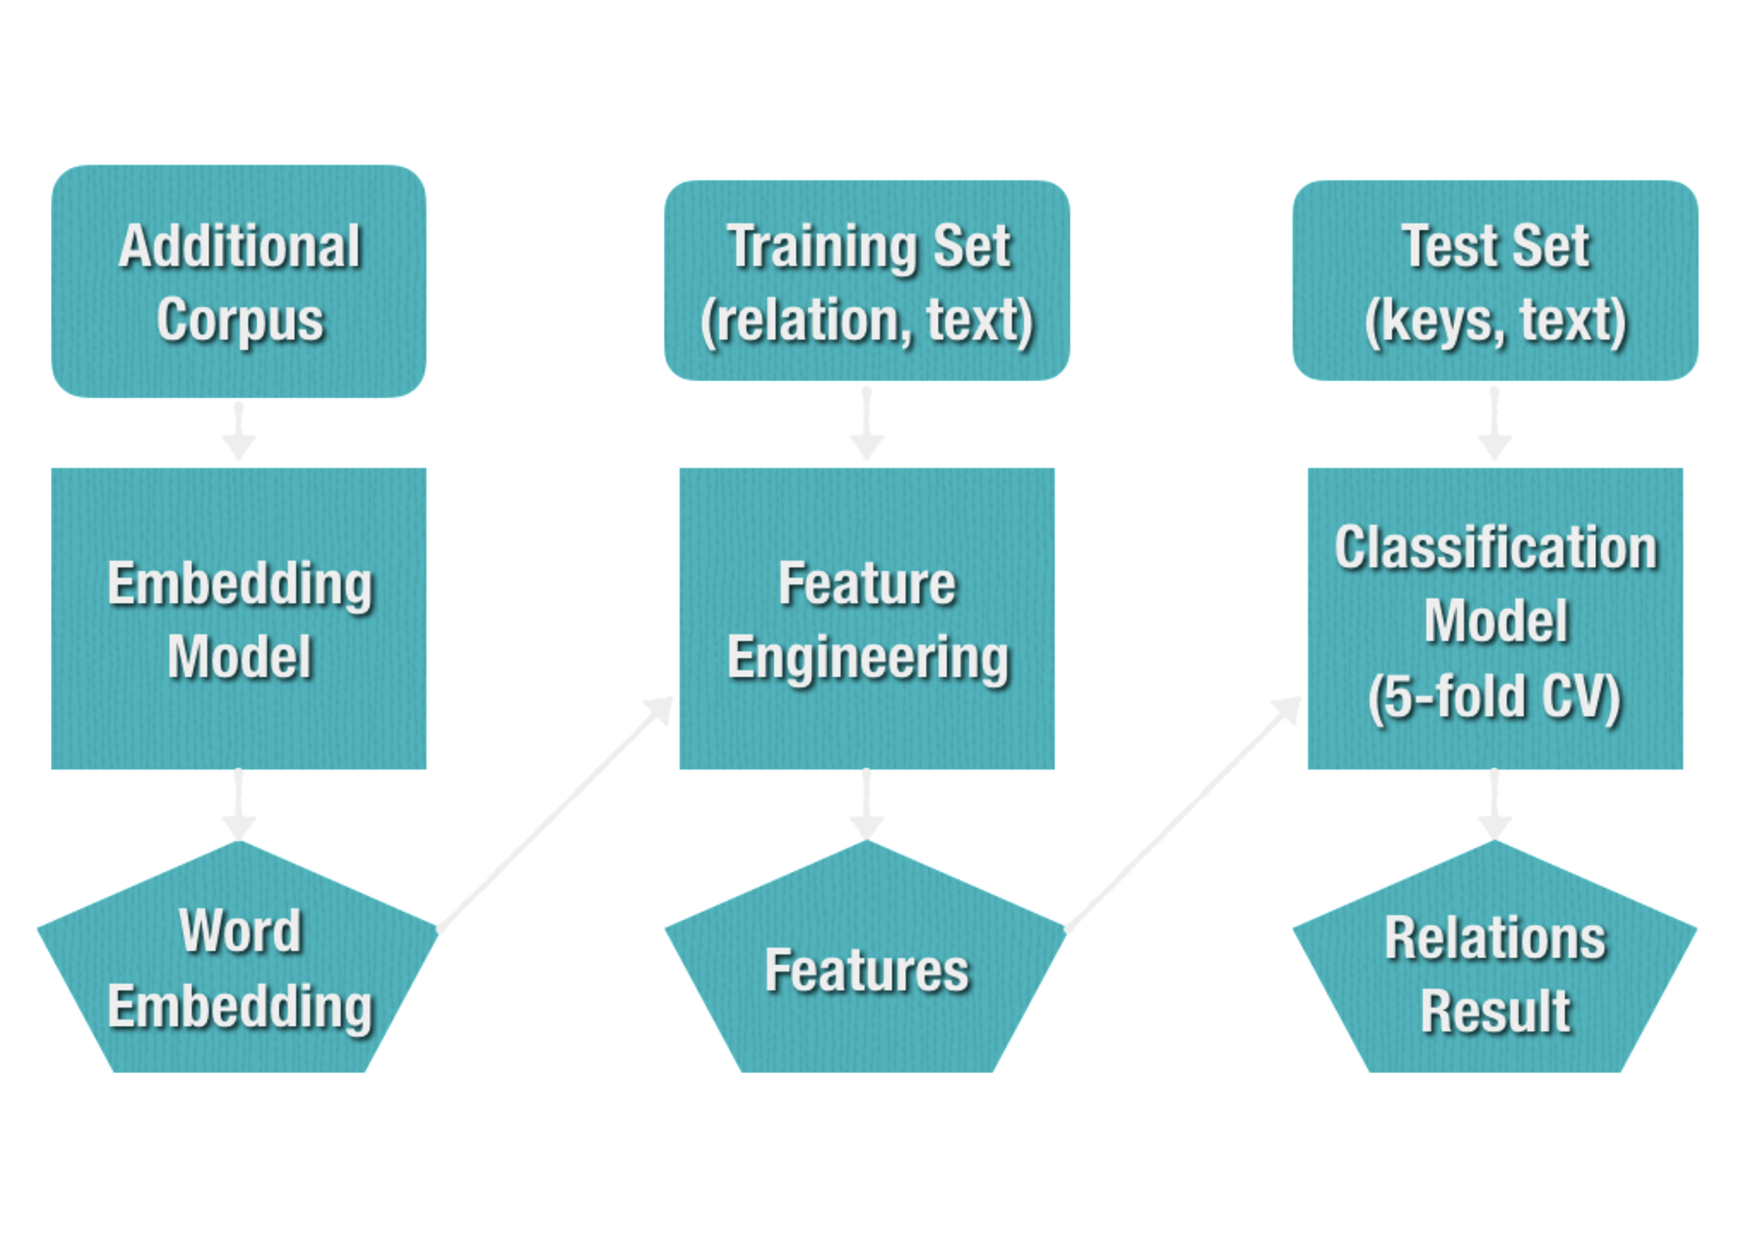
\includegraphics[width=0.85\textwidth]{figures/overall_model.pdf}
    \end{center}
    \caption{The overview of model structure}
    \label{fig:overall_model}
\end{figure*}
